\documentclass[TeamE-eindrapport]{subfiles}

\begin{document}
	
\chapter*{Inleiding}

	Dit is het eindverslag van de teamopdracht, waar we met alle leden van team \(\exists\)uler gedurende 9 weken aan gewerkt hebben. We maakten doorheen de sessies kennis met machine learning en we verwierven week na week meer en meer kennis over dit interessante onderwerp. We oefenden eerst op het onder de knie krijgen van twee basistechnieken, waarna we in week 6 begonnen met het uitwerken van onze eigen machine learning toepassing.
	
	\section*{Inhoud van dit eindverslag}

	We zullen in dit eindverslag de lezer eerst laten ontdekken wat machine learning precies is. Vervolgens bespreken we wat supervised learning inhoudt, in vergelijking met unsupervised learning. We bespreken ook wat classificatie juist is. Hierna zullen we het principe achter Support Vector Machines, de toepassing waarvoor we kozen, uitleggen. Hierbij zullen we verschillende classificatietechnieken vergelijken en beargumenteren waarom voor de tumor-dataset SVM een geschikte keuze blijkt te zijn.
	
	\section*{De gegevens}
	
	We maken in ons verslag gebruik van de resultaten van een onderzoek naar de verschillende eigenschappen van tumoren bij borstkankerpatiënten. Hierbij onderzochten wetenschappers W. Nick Street, W. H. Wolberg, en O. L. Mangasarian \cite{tumoronderzoek} in 1993 welke kenmerken het meest invloed hadden in het al dan niet kwaadaardig zijn van een tumor. Deze kenmerken werden berekend op basis van een gedigitaliseerd beeld van een fijne naaldaspiraat (FNA) van de borstmassa. Dergelijke beelden zijn te zien in figuur \ref{fig:borstscan}. De data die in het onderzoek vergaard werd, werd nadien publiek vrijgegeven \cite{tumordataset}, wat ons in de mogelijkheid stelt om de data te verwerken met hedendaagse Machine Learning technologie.
	
	\begin{figure}
		\hfill
		\subfloat{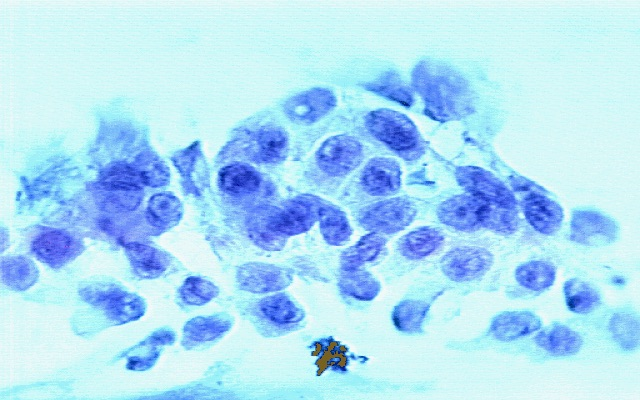
\includegraphics[width=4.5cm]{borstscan2}}
		\hfill
		\subfloat{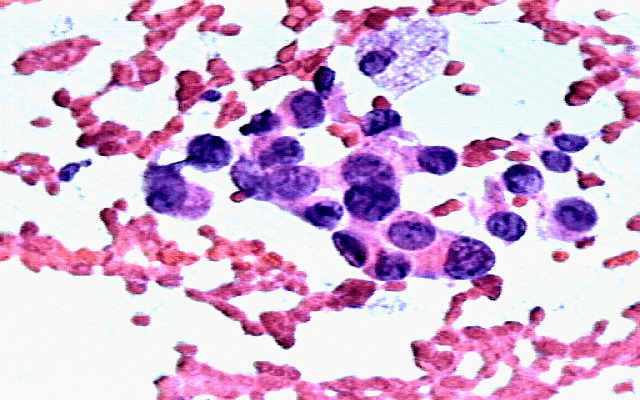
\includegraphics[width=4.5cm]{borstscan}}
		\hfill
		\subfloat{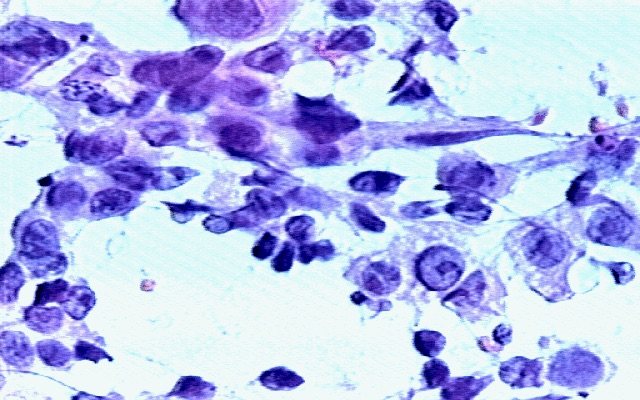
\includegraphics[width=4.5cm]{borstscan3}}
		\hfill
		\caption{Gedigitaliseerde beelden van fijne naaldaspiraten van de borstmassa.}
		\label{fig:borstscan}
	\end{figure}
	
\end{document}